\documentclass[10pt]{beamer}

%  {{{ Handout Generation

% \documentclass[10pt,handout]{beamer}
% \usepackage{pgfpages}
% \pgfpagesuselayout{4 on 1}[a4paper, landscape, border shrink=5mm]
% \pgfpageslogicalpageoptions{1}{border code=\pgfusepath{stroke}}
% \pgfpageslogicalpageoptions{2}{border code=\pgfusepath{stroke}}
% \pgfpageslogicalpageoptions{3}{border code=\pgfusepath{stroke}}
% \pgfpageslogicalpageoptions{4}{border code=\pgfusepath{stroke}}

% }}}
% {{{ Packages

\usepackage{soul}
\usepackage{amsmath}
\usepackage{todonotes}
\usepackage{graphicx}
\usepackage{xcolor}
\usepackage{nicefrac}
\usepackage{relsize}
% \usepackage{enumitem}
% \usepackage[
% 	%backend=biber, %instead of bibtex
% 	backend=biber,bibencoding=ascii,%
% 	language=auto,%
% 	style=nejm,%
% 	%style=authoryear-comp, % Author 1999, 2010
% 	%bibstyle=authoryear,dashed=false, % dashed: substitute rep. author with ---
% 	sorting=nyt, % name, year, title
% 	maxbibnames=10, % default: 3, et al.
% 	%backref=true,%
% 	natbib=true, % natbib compatibility mode (\citep and \citet still work)
% 	doi=true, isbn=false, url=false
% ]{biblatex}
\usepackage{pgfplots}
\usepackage{tikz}
\usetikzlibrary{shapes}
\usetikzlibrary{math}
\usetikzlibrary{calc}
\usetikzlibrary{patterns}
\usetikzlibrary{shapes,arrows,positioning,decorations.markings}
\usetikzlibrary{decorations.pathmorphing, decorations.text}
\usepackage{bm}
\usepackage[no-math]{fontspec}
\usepackage{fontawesome}
\newfontfamily{\FA}{FontAwesome}
\def\faThumb{{\FA \symbol{"F087}}}
\def\faGithub{{\FA \symbol{"F09B}}}
\def\faPlanet{{\FA \symbol{"F0AC}}}
\def\faPlus{{\FA \symbol{"F055}}}

\definecolor{KTHBlue}{HTML}{003C9E}
\definecolor{DarkGreen}{HTML}{526B0B}
\definecolor{DarkRed}{HTML}{AB2511}
\definecolor{LightRed}{HTML}{F73619}
\definecolor{DarkOrange}{HTML}{D16415}
\definecolor{Teal}{HTML}{0ABDC7}

\renewcommand{\footnotesize}{\scriptsize}

% }}}
% {{{ Theming
\usetheme[progressbar=frametitle]{metropolis}
% \usefonttheme[onlymath]{serif}

\setbeamercolor{normal text}{%
	fg=black!90,
	bg=black!2
}
\setbeamercolor{alerted text}{%
	fg=KTHBlue,
	bg=black!2
}
\setbeamerfont{alerted text}{
	series=\bfseries
}
\setbeamercolor{palette primary}{%
	use=normal text,
	fg=normal text.bg,
	bg=KTHBlue
}
\setbeamercolor{progress bar in head/foot}{fg=KTHBlue, bg=KTHBlue!10}
\setbeamercolor{progress bar in section page}{fg=KTHBlue, bg=KTHBlue!10}
\setbeamercolor{title separator}{fg=KTHBlue}

\AtBeginSubsection{\frame{\subsectionpage}}


% }}}
% {{{ Title Page

\title{Assemblées Générales 2017}
\subtitle{\^{}(Extra)?ordinaire\$}
\author{HAUM}
\date{6 Février -- Le Mans Innovation}
\institute{}
\titlegraphic{\begin{tikzpicture}[overlay]
	% \draw (10.0,-.5) node {\includegraphics[height=1.5cm]{logos/logolmi.png}};%
	\draw (10.4,-8.2) node {
\includegraphics[height=.8cm]{logos/logohaum.png}};%
\end{tikzpicture}}
% {{{ Custom Commands

\newcommand\cRed{\textcolor{DarkRed}}
\newcommand\cBlue{\textcolor{KTHBlue}}
\newcommand\cGreen{\textcolor{DarkGreen}}
\newcommand\cOrange{\textcolor{DarkOrange}}

\newcommand\etc{\textit{etc.}}
% \newcommand\bm{\mathbf}
\newcommand\del{\delta}
\newcommand\dd{~\mathsf{d}}
\newcommand\ff{\mathbf{f}}
\newcommand\FF{\mathbf{F}}
\newcommand\RR{\mathbf{R}}
\newcommand\CC{\mathbf{C}}
\newcommand\bT{\mathbf{T}^T}
\newcommand\bS{\mathbf{S}}
\newcommand\QQ{\mathbf{Q}}
\newcommand\PP{\mathbf{P}}
\newcommand\DDfull{\bm{b}(\partial_x\ff,\partial_y\ff)}

\newcommand{\btVFill}{\vskip0pt plus 1filll}
\renewcommand\div{\nabla\cdot}
\newcommand\hsigma{\hat{\sigma}}
\newcommand\Phat{\hat{P}}
\newcommand\Ahat{\hat{A}}
\newcommand\SV{\bm{s}}
\newcommand\vz{(z)}
\newcommand\tl\tilde
\newcommand\Td{\bm{T}(d)}
\newcommand\II{\bm{I}}

% }}}
% {{{ Graphics
% }}}
% \bibliography{CFM2017}
\begin{document}

% {{{ Title and TOC
\maketitle

\begin{frame}[standout]
	Assemblée Ordinaire
\end{frame}

\begin{frame}{Contenu}
	\setbeamertemplate{section in toc}[sections numbered]
	\tableofcontents[hideallsubsections]
\end{frame}
%  }}}

\section{Présentation de l'asso}
\section{Rapport moral}

\subsection{Le Mans Innovation}
\begin{frame}{Le Mans Innovation}
	\begin{itemize}
		\item Nouvelle adresse au 57 Bd. Demorieux (Le Mans, ici quoi.)
		\item 120m\textsuperscript{2}, 2 salles (1 propre, 1 sale)
		\item Nouveaux équipements:
			\begin{itemize}
				\item Découpeuse LASER Robotseed 600x400mm
				\item Ultimake 2+ Extended
			\end{itemize}
		\item Free coffee !
	\end{itemize}
\end{frame}

\begin{frame}{Le Mans Innovation -- Partenariats}
	Aujourd'hui 2 entreprises :

	\begin{itemize}
		\item Chaines de Pluie (Bertrand)
		\item Furion Motorcycles (Marc)
	\end{itemize}

	Et demain ?

	Besoin de prendre en compte leurs besoins aussi.
\end{frame}

\begin{frame}{Le Mans Innovation -- Quelques soucis}
	\begin{itemize}
		\item Accès non contrôlé (patché par note de service)
		\item Vers un fix: badges + gâche électrique
		\item Nécessité d'être fermes \& auto-régulé :
	\end{itemize}

	\pause
	\begin{center}
		Pas membre/Pas formé $\Rightarrow$ pas d'accès
	\end{center}
\end{frame}

\subsection{Évènements}

\begin{frame}{Évènements -- 24h du Code}
	\begin{itemize}
		\item Un sujet proposé en 2017 (énigmes en boule)
		\item Un sujet aussi en 2018 (Marabunta)
		\item Merci \textbf{beaucoup} à Florent, Laurent \& Corentin
		\item Bonne ambiance \& sympa
	\end{itemize}
\end{frame}

\begin{frame}{Évènements -- HAMExpo}
	\begin{itemize}
		\item Convention radioamateur sur Le Mans
		\item Rencontre avec l'Électrolab
	\end{itemize}
\end{frame}

\begin{frame}{Évènements -- Teriaki}
	\begin{itemize}
		\item 2 projets:
			\begin{itemize}
				\item Féroce: Labyrinthe 2D
				\item dHAUMadi : Simon says grandeur nature
			\end{itemize}
		\item Moins grosse fréquentation : soleil
		\item Bons contacts
	\end{itemize}
\end{frame}

\begin{frame}{Évènements -- Festival D}
	\begin{itemize}
			\item Nouvelle présentation de dHAUMadi
			\item Bon contacts et notamment
				\begin{itemize}
					\item Chemillé : dHAUM \& tricoteuse ?
					\item MyHumanKit : capteur myoélectrique libre
				\end{itemize}
			\item Qui organise 2019 ?
	\end{itemize}
\end{frame}

\begin{frame}{Évènements -- Jeudi du Libre}
	\begin{itemize}
		\item Redéfinition à l'AG 2017
		\item Échec partiel puis total à la cession
		\item Vers une nouvelle formule ?
	\end{itemize}
\end{frame}

\subsection{Projets et Axes}

\begin{frame}{Axes}
	\begin{description}
		\item[Photographie] Sténopé, stéréo-photographie, etc\ldots
		\item[Lumière] Plusieurs projets également : scratch holograms, light painting,  moirés, Tål
		\item[IdiHAUM\footnotemark]\footnotetext{Nom non définitif} Solution de contrôle d'accès
	\end{description}
\end{frame}

\subsection{Objectifs}

\begin{frame}{Objectif}
	\begin{itemize}
		\item Projets techniques, hackers contents
		\item Projets à deadline, hackers crevés
		\item HackPairHAUM
		\item HackerCamp (nhc18.org)
		\item Festival D
	\end{itemize}
\end{frame}

\begin{frame}[standout]
	Questions ?
\end{frame}

\begin{frame}[standout]
	On approuve ?
\end{frame}

\section{Rapport Financier}

\begin{frame}{En Images}
	\center
	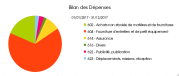
\includegraphics[width=\linewidth]{../convocation/2DossierAGDepenses2017.png}
\end{frame}

\begin{frame}{En Images}
	\center
	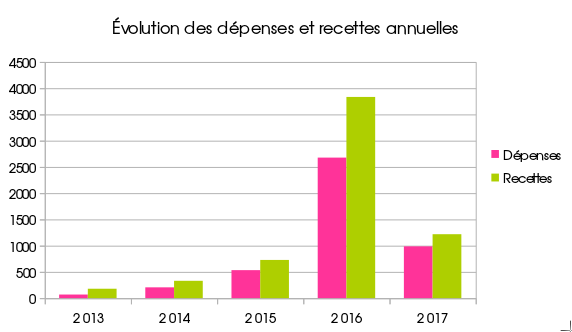
\includegraphics[width=\linewidth]{../convocation/3DossierAGGeneral2017.png}
\end{frame}

\begin{frame}{En Images}
	\center
	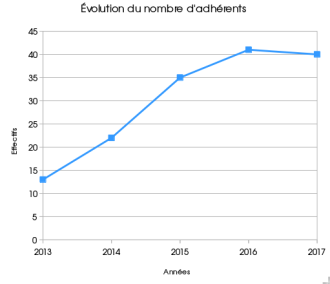
\includegraphics[width=\linewidth]{../convocation/4DossierAGAdherents2017.png}
\end{frame}

\begin{frame}{Bilan \& Objectifs}
	\begin{itemize}
		\item Bonne mutualisation \& nouveau matériel: Kress, tricoteuse, etc...
		\item Plus de machines ? Plus de cotis'
	\end{itemize}
\end{frame}

\begin{frame}{Bilan \& Objectifs}
	Deux trois règles :

	\begin{itemize}
	 \item toutes les factures doivent être établies \textbf{au nom du HAUM} et ne
	 contenir que des éléments \textbf{achetés pour le HAUM} ;
	 \item les dépenses de l'argent du hackerspace ne doivent être faites qu'après
	 \textbf{consultation des autres membres} et, surtout, \textbf{vérification de la
	 trésorerie} ;
	 \item une demande de validation \textbf{par mail} doit être effectuée.
	\end{itemize}
\end{frame}

\begin{frame}[standout]
	Questions ?
\end{frame}

\begin{frame}[standout]
	On approuve ?
\end{frame}

\section{Questions diverses}

\begin{frame}{Questions diverses}
	\begin{itemize}
		\item Hacker profiles (matael pour feedoo)
		\item Liste du matériel sur le site (seb)
	\end{itemize}
	\vfill
	\begin{center}
		\large
		D'autres questions à aborder ?
	\end{center}
\end{frame}

\section{Élection du bureau}

\begin{frame}[standout]
	Assemblée extraordinaire
\end{frame}

\begin{frame}[standout]
	Réunion du bureau
\end{frame}

\begin{frame}[standout] % Thank you
	\vspace{0.05\textwidth}
	Merci !\\
	\vspace{0.25\textwidth}
	\small{\texttt{gaborit@kth.se}}\\
\end{frame}

\end{document}
% vim: spelllang=fr
